\documentclass[12pt]{article}
\usepackage{amsmath}
\usepackage{listings}
\usepackage{xcolor}
\usepackage{float}
\usepackage{url}

\definecolor{codegreen}{rgb}{0,0.6,0}
\definecolor{codegray}{RGB}{4,118,219}
\definecolor{codepurple}{rgb}{0.58,0,0.82}
\definecolor{backcolour}{RGB}{0,27,51}
\definecolor{textcolour}{RGB}{38, 149, 245}

\lstdefinestyle{mystyle}{
    backgroundcolor=\color{backcolour},   
    commentstyle=\color{codegreen},
    keywordstyle=\color{magenta},
    numberstyle=\tiny\color{codegray},
    stringstyle=\color{codepurple},
    basicstyle=\ttfamily\color{textcolour}\footnotesize,
    breakatwhitespace=false,         
    breaklines=true,                 
    captionpos=b,                    
    keepspaces=false,                 
    numbers=left,                    
    numbersep=5pt,                  
    showspaces=false,                
    showstringspaces=false,
    showtabs=false,                  
    tabsize=2
}

\usepackage{setspace}
\onehalfspacing
%\doublespacing

\lstset{literate=%
    {Ö}{{\"O}}1
    {Ä}{{\"A}}1
    {Ü}{{\"U}}1
    {ß}{{\ss}}1
    {ü}{{\"u}}1
    {ä}{{\"a}}1
    {ö}{{\"o}}1
    {~}{{\textasciitilde}}1
}

\lstset{style=mystyle}

    \title{\textbf{Bachelorarbeit}}
    \author{Jan Philipp Fortowski}
    \date{xx.xx.2024}
    
    \addtolength{\topmargin}{-3cm}
    \addtolength{\textheight}{3cm}
\usepackage{graphicx}
\begin{document}


\maketitle
\cleardoublepage
% \phantomsection
\tableofcontents
\cleardoublepage
% \phantomsection
\thispagestyle{empty}



\section{Pooling Layer}
Pooling Layer werden dazu verwendet, um das sogenannte Downsampling zu betreieben. Downsampling bedeutet einfach, dass eine geringere Auswahl an Daten weitergegeben werden.
In einem Netzwerk benutzt man eines dieser Verfahren, um die weiteren Schichten nur mit den nötigsten Daten zu belasten. Gerade in Anbetracht der Größe der Daten, die bei den Convolutional Layern entstehen, kann das viel Zeit sparen. Aber Hauptsächlich sorgt dies auch dafür, dass das Netzwerk weniger anfällig für Veränderungen der Daten wird. leichte Veränderungen der Daten können für gravierende Änderungen, das heißt wenn ein Bild nicht korrekt Zentriert ist, oder wenn es um ein paar Grad gedreht wird, kommt ein Netzwerk schnell durcheinander.
Die Convolution Layer erstellen Feature Maps, in denen die Features allerdings auch die gleichen Positionen haben, wie in den Inputs. Dadurch können bei kleinen Veränderungen schon Fehler in den nächsten Schichten entstehen. Dem kann man durch das Downsampling entgegenwirken.

Auf eine Gewisse weise können die Daten bereits in den Convonlutional Layern "gedownsampelt" werden, wenn die Schrittgröße (Stride) beim anwenden der Filter Größer ist als 1.

Wie genau Funktioniert ein Pooling Layer dann? so wie bei den Convolutional Layern werden Filter eingesetzt. Diese sind aber kleiner, und funktionieren anders. Meist ist ein Filter hier nur 2x2 groß, und bei der Anwendung wird eine Schrittgröße von 2 verwendet. Die Filter überlappen die Felder nicht, die bereits behandelt wurden. 
Auf die Pixel, auf die der Filter angewand wird, werden nun eine Pooling Operation angewand. 

Zwei mögliche Pooling Operationen sind das Durschnitts Pooling und das Maximum Pooling. 
\begin{itemize}
  \item Das Durchschnitts Pooling gibt den Durchschnitt aller Werte als Output zurück, während
  \item das Maximum Pooling nur den Größten Wert der betrachteten Werte zurückgibt.
\end{itemize}
Es gibt noch weitere, wie zum Beispiel das Globale Pooling, bei dem die Gesammte Feature Map auf einen einzigen Wert reduziert wird. Dadurch soll auf eine möglichst Aggressive Art festgestellt werden, ob ein bestimmtes Feature überhaupt in der Feature Map vorkommt. Je nach Anwendungsfall kann auch diese Methode erfolg bringen.




\section{Unterstützungs Templates}
Die Gliederung dieser Arbeit, entspricht einer organischen Herangehensweise oder einer Anleitung, wie ein Netzwerk aufgebaut wird. Jedes Kapitel entspricht einem Teil des Netzwerkes, also den Funktionen, der Initialisierung, der Query oder Abfrage und dem Lern- oder Backpropagation-Algorithmus. Jedes der Kapitel startet mit einer Übersicht, über die Funktionalität, erläutert die Theorie dahinter, teilweise auch mathematisch, und schließt, mit dem daraus resultierenden Code ab. 


\begin{figure}[H]
\centering
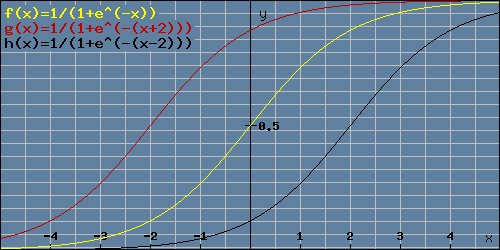
\includegraphics[scale=0.60]{./Images/Pasted image 20231005145933.png}
\caption{Sigmoidfunktion mit Bias}
\label{Sigmoid-Funktion mit Bias}
\end{figure}


\begin{itemize}
  \item Dendriten
  \item der Zellkörper
  \item das Axon
\end{itemize}

\begin{lstlisting}[language=Java]
public class NeuralNetwork {
    Layer[] layers;
    double learnRate;    // Initialisierung
    public NeuralNetwork(double learnRate, int... layerSizes) {
        layers = new Layer[layerSizes.length - 1];
        for (int i = 0; i < layers.length; i++) {
            layers[i] = new Layer(layerSizes[i], layerSizes[i + 1]);
        }
        this.learnRate = learnRate;
    }
}
\end{lstlisting}

Aber verfolgen wir diesen Gedanken doch einmal an einem Beispiel:
Sei $f(w)$ unsere Funktion: $$f(w)=w^2+3$$
Wir nennen die kleine Verschiebung von $w$ jetzt $h$.
Dann gilt zumindest schon einmal: $$\Delta w=(w+h)-w$$Und gekürzt:$$\Delta w=h$$
Dann wäre die Änderungsrate also:$$\ddot{A}nderungsrate = \frac{\Delta e}{\Delta w}$$ $$\frac{\Delta e}{\Delta w}=\frac{f(w+h)-f(w)}{h}$$
Wenn wir uns dann die Mühe machen, $f(w)$ aus zuschreiben, ergibt sich daraus:
$$\frac{\Delta e}{\Delta w}=\frac{(w+h)^2+3-(w^2+3)}{h}$$
Dann fangen wir an Klammern auszurechnen:
$$\frac{\Delta e}{\Delta w}=\frac{w^2+w*h+w*h+h^2+3-w^2-3}{h}$$
$$\frac{\Delta e}{\Delta w}=\frac{w^2+w*h+w*h+h^2-w^2}{h}$$
$$\frac{\Delta e}{\Delta w}=\frac{w*h+w*h+h^2}{h}$$
$h$ kürzen:
$$\frac{\Delta e}{\Delta w}=w+w+h$$
$$\frac{\Delta e}{\Delta w}=2w+h$$Und jetzt zum Interessanten Teil. Da wir $h$ nicht gleich 0 setzten können, können wir allerdings $h$ gegen 0 laufen lassen, dann verwenden wir die Leibniz-Notation. Das bedeutet, dass wir anstatt  $\Delta w$ und  $\Delta e$, wobei $\Delta$ eine sehr kleine Vergrößerung darstellt, jetzt $dw$ und $de$ verwenden, wobei $d$ für eine unendlich kleine Vergrößerung steht, eine sogenannte Infinitesimalzahl.
Das sieht dann ungefähr so aus:
$$\frac{de}{dw}=\lim_{h\to 0} 2w +h$$
$$\frac{de}{dw}=2w$$








\section{Einleitung}
\subsection{Motivation}
Neuronale Netzwerke werden vor allem für Klassifikationsverfahren verwendet. In der Praxis gibt es viele Anwendungsbereiche, in denen es vorteilhaft ist, große Mengen von Daten automatisch zu klassifizieren. Einige Beispiele, wären die Bild- und Schrifterkennung, die man dazu verwendet, Kennschilder von Autos, maschinell auszulesen. Solche Technologien werden immer häufiger auf Parkplätzen und Autobahnen eingesetzt. Aber, auch fast jedes Handy kann mittlerweile Schrift erkennen, die mit der Kamera aufgenommen wird. Auch in der Medizin, beim Auswerten von Röntgenbildern, in der Biologie, zum Erkennen von Pflanzen auf Fotos und noch vielem mehr, werden Neuronale Netzwerke inzwischen eingesetzt.\\
Es gibt kaum einen Bereich, in dem sich nicht eine mögliche Anwendung für Neuronale Netzwerke finden lässt. Ganz besonders aufwändige Netzwerke, werden mittlerweile auch für konstruktive Aufgaben verwendet, wie zum Beispiel Sprachmodelle, unter anderem ChatGPT und Bilder generierende KIs, wie Midjourney.
Typische Probleme, bei welchen neuronale Netzwerke eingesetzt werden, sind komplexe Aufgaben, mit gigantischen Datenmengen.\\
Eine Aufgabe ist zu komplex, wenn eine Lösung nicht manuell programmiert werden kann, unter anderem, bei der Bilderkennung. Außerdem sollten solche Probleme automatisiert werden, weil es sich nicht lohnt, Menschen dazu einzusetzen. 
In solchen Fällen, werden neuronale Netzwerke eingesetzt.\\
Im Laufe der Zeit sind die modernen Netzwerke immer komplexer geworden und liefern nahezu menschliche Ergebnisse, im Bruchteil der Zeit, die Menschen dafür brauchen würden. Aber wie genau funktioniert so ein Netzwerk?



\cleardoublepage
% \phantomsection
\sloppy
\section{Quellen}
\begin{itemize}
\item 1. B. Lenze, Einführung in die Mathematik neuronaler Netze. Berlin: Logos Verlag; 2009.
\item 2. T. Rashid, Neuronale Netze selbst programmieren - Ein verständlicher Einstieg mit Python. Paderborn: O’Reilly Verlag; 2017.
\item 3. S. Lague, How to Create a Neural Network (and Train it to Identify Doodles). Hrsg. auf dem YouTube Kanal [Sebastian Lague](\url{https://www.youtube.com/@SebastianLague}). Ohne Jahr [zitiert am 16. September 2023]. Abrufbar unter: URL: \url{https://www.youtube.com/watch?v=hfMk-kjRv4c}.
\item 4. "Ableitung der Sigmoid-Funktion" URL: \url{https://ichi.pro/de/ableitung-der-sigmoid-funktion-91708302791054}
\item 5. "What is the role of the bias in neural networks?" URL: \url{https://stackoverflow.com/questions/2480650/what-is-the-role-of-the-bias-in-neural-networks}.
\item 6. "How do I choose the optimal batch size?", URL: \url{https://ai.stackexchange.com/questions/8560/how-do-i-choose-the-optimal-batch-size}
\end{itemize}

\cleardoublepage
\section{Liste der Abbildungen}
\listoffigures
\end{document}